\chapter[Execução à nível de Portfólio]{Execução à nível de Portfólio}
Esse tópico representa as atividades e resultados obtidos pela equipe durante a execução do processo definido a nível de portfólio.

\begin{figure}[H]
    \centering
    \label{identificarInteresse}
    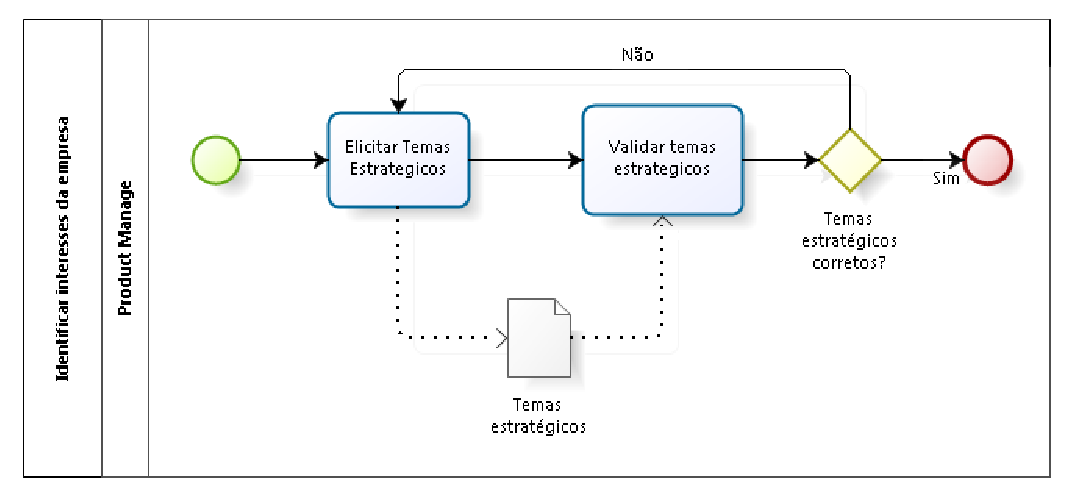
\includegraphics[keepaspectratio=true,scale=0.6]{figuras/processoInteresses.eps}
    \caption[Identificar interesses da empresa]{Processo - Nível de Portfólio - Identificar interesses da empresa}
\end{figure}

\begin{figure}[H]
    \centering
    \label{identificarInteresse}
    \includegraphics[keepaspectratio=true,scale=0.6]{figuras/processoValores.eps}
    \caption[Identificar valores da empresa]{Processo - Nível de Portfólio - Identificar valores da empresa}
\end{figure}

\section{Reuniões realizadas}
Foram realizadas duas reuniões, entre a equipe e o cliente, para obter as informações necessárias à nível de portfólio, sendo a primeira reunião, presencial e segunda, não presencial.
\subsection{Reunião 01-Portfólio}\label{Reunião01-Portfólio}

\indent \textbf{Data de execução:} 12/05/2016.\\
\indent \textbf{Objetivo da reunião:} entender o contexto de negócio, entender a problemática da empresa, elicitar os temas estratégicos e épicos de negócio.\\
\indent \textbf{Técnica de elicitação:} entrevista aberta, consiste em o entrevistador, membro da equipe de requisitos, possibilitar ao entrevistado, o Product Owner, expor as suas ideias a respeito do tema em questão \cite{leffingwell2011}, no caso, o problema da empresa.\\
\indent \textbf{Execução da técnica:} antes da reunião, foi elaborada perguntas para que objetivo da reunião fosse alcançado. Na execução desta, foi geradas mais perguntas a medida que a equipe entendia o problema. Sendo devidamente documentadas, representado pelo apêndice: ???.\\
\indent \textbf{Resultado da reunião:} ao término da reunião foram obtidos, o diagrama de causa e efeito, representando o problema principal da empresa e seus sub problemas, este que será explanado na imagem \ref{fishBone}. O tema estratégico e o épico de negócio da empresa, estão representados na imagem: \ref{backlogTemaEpicoImg}.\\

\subsection{Reunião 02-Portfólio}\label{Reunião02-Portfólio}

\indent \textbf{Data de execução:} 27/05/201.\\
\indent \textbf{Objetivo da reunião:} validar os temas estratégicos e os épicos de negócio elicitados com o PO, confirmar com este se os épicos e temas, estavam de acordo com seus interesses e suas necessidades. Devido o fato de só existir um tema estratégicos \ref{tema1} identificado, o segundo objetivo da reunião foi fazer a priorização dos épicos.\\
\indent \textbf{Resultado da reunião:} ao término da reunião foram obtidos, o diagrama de causa e efeito, representando o problema principal da empresa e seus sub problemas, será explanado na imagem \ref{fishBone}. O tema estratégico e o épico de negócio da empresa, representado no \ref{backlogTemaEpicoImg}.\\

\section{Entendimento do problema}
A Zenit Aerospace é uma empresa júnior, da Univerdade de Brasília - Campus gama. A empresa é mantida pelos próprios alunos, em sua maioria são alunos de graduação da engenharia aeroespacial

\subsection{Organização da empresa}
Atualmente é dividida em dois tipos de funcionários: gestores e assessores. Os cargos de gestão são delegados a estudantes que são incorporados a empresa, cuja função é coordenar, gerir, controlar, uma das cinco diretorias ou a presidência da empresa. Aqueles que não estão no cargo de gerência são assessores, em que a responsabilidade é assessorar, auxiliar, dar suporte aos gestores. Ressalta-se que a participação no desenvolvimento de projetos não é restrita.

\begin{figure}[H]
    \centering
    \label{organizacaoZenit}
    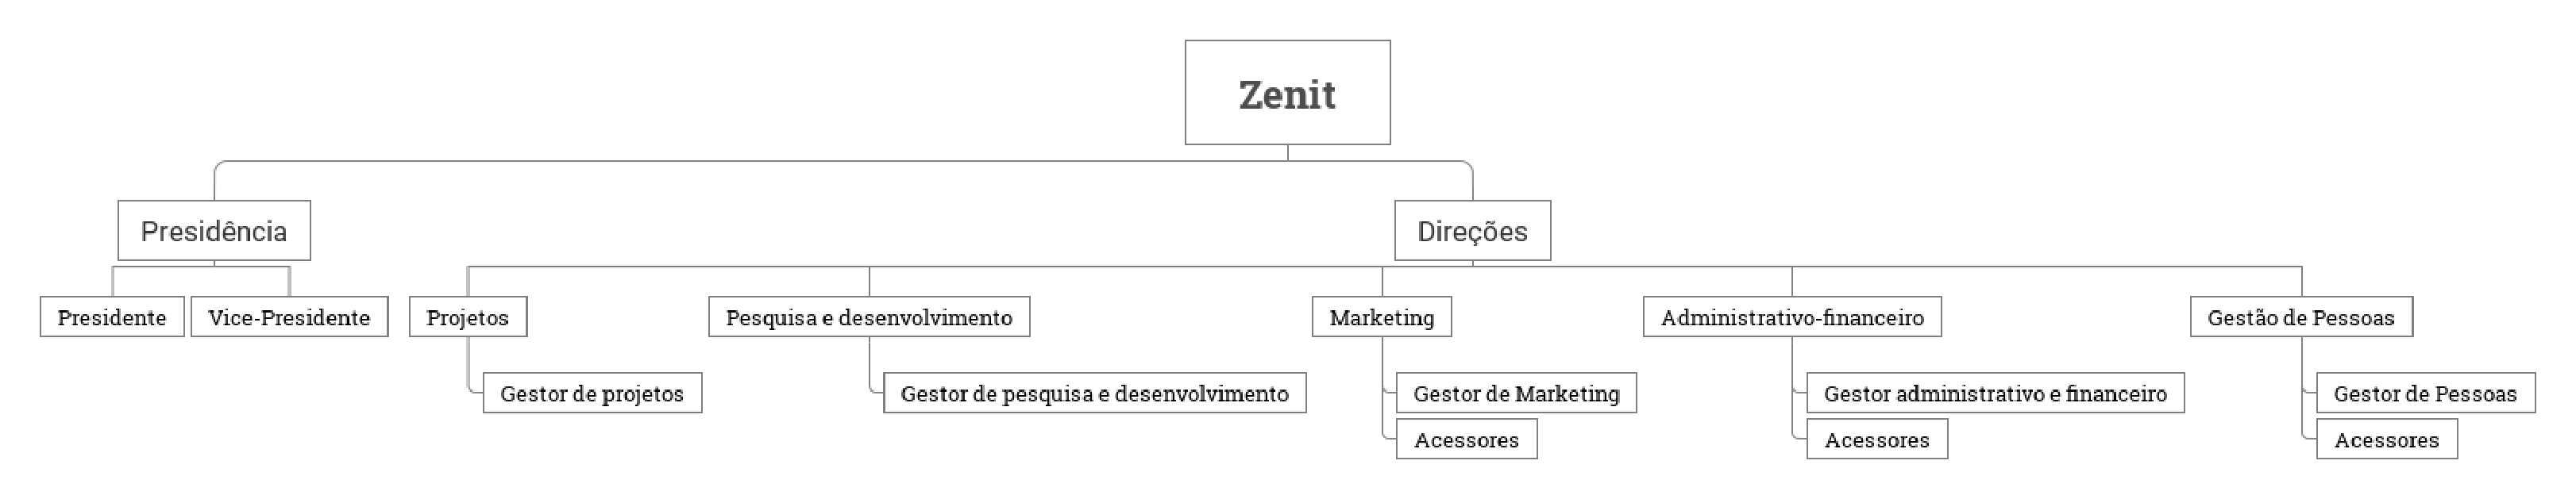
\includegraphics[keepaspectratio=true,scale=0.3]{figuras/zenitOrganograma.eps}
    \caption[Organização da empresa]{Organização da empresa}
\end{figure}

As demais direções executivas são: Presidência, Gestão de Pessoas, Marketing, Administrativo-financeiro, Projeto e Pesquisa e desenvolvimento. 

A direção de pessoas é responsável por supervisionar a atualização do banco de dados de membros da empresa, prover a motivação dos membros mediante políticas de reconhecimento, emissão de certificados da participação dos membros em projetos, auxiliar no planejamento de treinamentos, seleção de membros para os projetos \cite{regimentoInternoZenit}.
A direção de projetos é responsável por gerir os projetos, trabalhos, demandas para a empresa. Esta área determinará a quantidade de pessoas a serem alocadas, as capacidades técnicas necessárias e juntamente com a direção de pessoas, quais funcionários possuem os requisitos para preencher a vaga no projeto \cite{regimentoInternoZenit}.

\section{Descrição do problema}
O gestor de pessoas é responsável por organizar os dados dos funcionários da Zenit com relação a sua capacitação e seus dados pessoais. A atual forma para manter os dados da empresa não atende a expectativa do gestor de pessoas, pois dificulta a utilização destes para o desempenho de suas atividades que necessite da informação dos funcionários. Há uma planilha online do Google Drive no qual todos os dados pessoais dos funcionários ficam registrados, porém não há o registro da capacitação de cada funcionário. Todos os membros recebem acesso, mas somente o gestor de pessoas e o presidente organizacional tem autorização de modificar algum dado. Caso algum funcionário saia da empresa, é responsabilidade do gestor de pessoas remover os dados do ex funcionário, assim como o acesso as informações dos demais funcionários.

Além disso o gestor de pessoas não consegue fazer acompanhamento das habilidades técnicas e experiências, e determinar com base nos dados de qualificação de cada membro quais são as atividades recomendáveis para ele desempenhar.

Tendo como base os resultados recolhidos pela equipe de requisitos na primeira reunião, o problema da organização foi representada pelo  diagrama de causa e efeito a seguir.

\begin{figure}[H]
    \centering
    \label{fishBone}
    \includegraphics[keepaspectratio=true,scale=0.3]{figuras/Inefici_ncia_na_gest_o_de_pessoas_p.eps}
    \caption[Diagrama de causa e efeito]{Diagrama de causa e efeito}
\end{figure}

A tabela a seguir foi feita para representar resumidamente o problema, a fim de possibilitar melhor entendimento do problema.

\begin{table}[H]
    \centering
    \label{descricaoAtividades}
    \caption{Problema}
        \begin{tabular}{|l|p{10cm}|}
        \hline
        \textbf{O problema da empresa é} &Ineficiência da gestão de pessoas.\\
        \hline
        \textbf{Afeta} &Os gestores da Zenit\\
        \hline
        \textbf{As consequências são} &Ineficiência de escolha de membros para os projetos e a desmotivação para realizar certas atividades dos membros.\\
        \hline
        \textbf{Uma solução bem sucedida seria} &Um sistema que centralizaria as informações dos membros da empresa e possibilita fazer buscas nestes dados.\\
        \hline
    \end{tabular}
\end{table}

\section{Backlog Porfólio}
O backlog a seguir foi elaborado a partir das reuniões com o \textit{Product Owner} até o presente momento da execução do processo. O backlog do apêndice \ref{backlogPortfolio} possui os temas estratégicos e épicos ao final da execução do processo, ou seja, contém mudanças que foram realizadas após esta etapa do relatório.


\subsection{Temas estratégicos}
\begin{itemize}
\item {TE01 - Conhecimento e acompanhamento individual dos membros da empresa}
\end{itemize}

\subsection{Épicos}
\textbf{Business}
\begin{itemize}
\item {EP01 - Informações sobre membros da empresa}
\item {EP02 - Acompanhamento do desempenho de membros da empresa}
\end{itemize}

\textbf{Enable:}
\begin{itemize}
\item {EP03 - Servidor para aplicação web}
\end{itemize}
